\chapter{最短路径算法实现}
\section{最短路径算法分析}
\par 在二维空间中,通常是基于二维垂直的欧几里得空间,其中x轴和y轴垂直,顶点通常以类似经纬度形式给出,如~(x,y)~代表该顶点分别该点坐标分别在x轴、y轴上的长度分量,点~(a,b)~在~x~轴的分量为~a~,在~y~轴的分量为~b~;其中顶点之间会与若干条路径相连,其中路径不能经过相关障碍物,路径的权值可以是该条路径的长度或该条路径所需费用,记为~W(i,j)~表示第~i~个顶点到第~j~个顶点的边的权值。例如在运输网络中,顶点代表的是不同城市的集散地,顶点之间的路径就是城市之间的交通网,路径的权值代表该条交通路线所需要的时间,则所求的顶点到顶点的最短路径即是最短时间的路线。
\subsection{基于Dijkstra算法的最短路径求解}
\par Dijkstra该算法基于贪心的思想,解决了图~G=<V,E>~上带权的单源最短路径问题,通过设置一顶点集合~S~,在集合S中所有的顶点与源点s之间的最终最短路径权值均已被计算出来。算法反复选择最短路径估计最小的点$u\in V-S$并将~u~加入到~S~中,最终计算出源点到其他所有点的最短距离。举例来说,若图中的顶点代表城市,而边上的权值表示城市间开车行车的距离,该算法可以用来找到两个城市之间的最短路径。但是Dijkstra算法并不能有效处理带有负权边的图。
\par 算法描述:Dijkstra算法通过保留目前为止所找到的每个顶点$v\in V$从~s~到~v~的最短路径来工作。初始时,原点s的路径权重被赋为0。同时把所有顶点的路径长度设为无穷大,即表示我们不知道任何通向这些顶点的路径。当算法结束后,~d[v]~中存储的便是从s到v的最短路径,或者如果路径不存在的话是无穷大。
\par 松弛操作是Dijkstra的基础操作:如果存在一条从u到v的边,那么从s到v的一条新路径是将边$w(u,v)\in E$添加到从s到u的路径尾部来拓展一条从s到v的路径。这条路径的长度是$d[u]+w(u,v)$。若这个值比目前已知的$d[v]$的值要小,那么可以用这个值来替代当前$d[v]$中的值。松弛边的操作一直运行到所有的$d[v]$都代表从s到v的最短路径的长度值。由于基于松弛操作,因此若存在负权值边中的负环时会重复松弛,导致无法正确求解出最短路径。
\par 算法维护两个顶点集合openList和clostList,集合openList保留所有已知实际最短路径值的顶点,而集合clostList则保留其他所有顶点。集合S初始状态为空,而后每一步都有一个顶点从Q移动到S。这个被选择的顶点是Q中拥有最小的$d[u]$值的顶点。当一个顶点~u~从~Q~中转移到了~S~中,算法对u的每条外接边$w(u,v)$进行松弛。
\par 算法的步骤如下
\begin{enumerate}
    \item 输入边全为正权的图,G中带有顶点V=$v_0,v_1,v_2\dots$和若干边$w(v_i,v_j)$
    \item 设置一个待检测列表clostList和一个不需检测列表clostList;
    \item 将起始点startPoint加入openList中;
    \item 初始化距离向量~d~,其中startPoint的距离为0,其他全为正无穷;
    \item 检测openList,找出~d~值最小的一个点,将此节点作为当前节点(curNode),并加入closeList中不再检测;
    \item 若该点等于终点endPoint,此时终止算法,已找到最短路径,返回该点的距离向量;
    \item 否则遍历curNode的相邻节点,若该节点是不可通过的、或在closeList中的、或超过边界的,则跳过;
    \item 保存该节点的parent为curNode,计算其距离向量值~d~,再保存到openList中;
    \item 若此时openList为空,算法结束,未找到起点到终点的最短路径;
    \item 若openList不为空,回到步骤5;
\end{enumerate}
\par 算法中的步骤8,计算相邻节点(Node)的距离向量~d~时,即是算法的松弛操作,具体计算方法是:$if (d[curNode] + w(curNode, Node) < d[Node]) d[Node] = d[curNode] + w(curNode, Node)$,通过不断的将所有点加入openList来松弛到其他顶点的距离向量,最后就能计算出从起点到终点的最短路径了。
\par 例如使用该算法来寻找两个城市之间的最短路径,整个图是城市之间的交通网,此时顶点是城市,顶点之间的路径是城市之间的交通路线,路径的权值是行驶所需的时间,因此两个城市之间可能有多条权值不同的路径,此时使用Dijkstra算法求解得到的最短路径即是从起点出发到其他顶点的所需要的最短时间的路线。
\subsection{基于A*算法的最短路径求解}
\par A*搜索算法综合了最良优先算法(Best-first search)和Dijkstra算法的优点:在进行启发式搜索提高算法效率的同时,可以保证找到一条最优路径(基于评估函数)。
\par 该算法中,以~g(n)~表示从起点到任意顶点n的实际距离,~h(n)~表示任意顶点n到目标顶点的估算距离,那么A*算法的估算函数为~f(n)=g(n)+h(n)~,这个公式遵循以下特性:
\begin{itemize}
    \item 如果~g(n)~为0,即只计算任意顶点n到目标的评估函数~h(n)~,而不计算起点到顶点n的距离,则算法转化为使用贪心策略的最良优先搜索,速度最快,但可能得不出最优解;
    \item 如果~h(n)~不大于顶点n到目标顶点的实际距离,则一定可以求出最优解,而且~h(n)~越小,需要计算的节点越多,算法效率越低,常见的评估函数有-欧几里得距离、曼哈顿距离、切比雪夫距离;
    \item 如果~h(n)~为0,即只需求出起点到任意顶点n的最短路径~g(n)~,而不计算任何评估函数~h(n)~,则转化为单源最短路径问题,即Dijkstra算法,此时需要计算最多的顶点。
\end{itemize}
\par 其步骤如下
\begin{enumerate}
    \item 设置一个待检测列表openList和一个不需检测列表clostList;
    \item 把起始点startPoint加入openList中;
    \item 检测openList,找出其中~f~值最小的一个点,将此节点作为当前节点(curNode),并加入closeList中不再检测;
    \item 若该点等于终点endPoint,此时终止算法,已找到最短路径;
    \item 否则遍历curNode周围的节点,若该节点是不可通过的、在closeList中的、超过边界的,则跳过;
    \item 保存该节点的parent,计算~f~值,再保存到openList中;
    \item 若此时openList为空,算法结束,未找到目的点;
    \item openList不为空,回到步骤3;
\end{enumerate}
\par A*算法通过启发式搜索,即评估函数~h(n)~,进一步提高了寻找最短路径的效率,减小了无用点的遍历过程,可以大大的节省时间和空间的消耗。
\section{三维最短路径}
\par 对于类似实际空间的三维空间,由于三维空间当中顶点的数量较多,且存在复杂的障碍物关系,使得在三维空间中求解最短路径算法对于空间复杂度和时间复杂度之间存在一定的受限,在三维空间当中求解最短路径更偏向于求解近似最短路径,以满足时间和空间的要求,因此算法主要解决在一定的精度误差内近似求解出给出起点到终点之间的最短路径长度及所经过的顶点路径。
假设空间离散时精度为~precision~,即代表实际空间中的1单位长度对应离散化空间的~precision~单位长度。
则在实际空间中的点坐标~(x,y,z)~可以离散化为格子点坐标$(\lfloor\dfrac{x}{precision}\rfloor,\lfloor\dfrac{y}{precision}\rfloor,\lfloor\dfrac{z}{precision}\rfloor)$,则我们需要对起点、终点和障碍物都完成离散化的过程,然后在离散化空间中求解起点到终点的最短路径。

\subsection{数据处理}
\par 首先,根据实际空间的障碍物,模型成若干个如图的长方体,其中长方体满足底面为一个矩形,但可能长宽不平行于x、y轴,高平行于三维空间的z轴。数据中会以实数给出底面矩形平行的两边的中点$M_0(a,b),M_1(c,d)$,与之垂直的边的长度~D~,以及该立方体的z轴范围$z_0,z_1$。通过给出的数据可以计算得出该长方体障碍物所对应的顶点。
根据实际空间模型,需要首先按照指定的精度将实际空间的模型划分到指定精度的空间,将空间划分为若干个离散化的格点,通过计算该精度下障碍物所经过的格子点,这些障碍物的离散格点都是在计算最短路径时不可以通过的。
\par 根据障碍物底面为一个矩形,其满足长与宽垂直,则设两中点$M_0,M_1$所在直线为矩形的长,则如图\ref{fig:obstacle_bottom},设该矩形的四个顶点分别为$A(x_0,y_0)$、$B(x_1,y_1)$、$C(x_2,y_2)$、$D(x_3,y_3)$且满足相邻的关系,根据$M_0M_1$直线的表达式,和$\vec{M_0A}\times\vec{M_0M_1}=0$可以计算出与之垂直的直线$M_0A$的表达式为:
$$
    y-b=\dfrac{d-b}{c-a}(x-a)
$$
设$k=\dfrac{d-b}{c-a}$,则原式为$y-b=k(x-a)$。且矩形的宽为~D~,则$d(M_0,A)=\frac{D}{2}$,故有$\sqrt{(a-x_0)^2+(b-y_0)^2}=\frac{D}{2}$。
将$y-b=k(x-a)$代入方程,可以得到与$M_0$相邻的顶点A、D的x坐标分别为
$$
    x=a\pm\dfrac{\frac{D}{2}}{\sqrt{k^2+1}}
$$
将计算出来的坐标代入$y-b=k(x-a)$可得该点对应的y坐标。相似地,计算与$M_1$相邻的两顶点时,将与$M_0M_1$的直线方程所经过的点$M_0$修改为$M_1$,即该直线方程为$y-c=k(x-d)$,类似的满足与$M_1$相邻的顶点B、C满足的x坐标的关系为
$$
    x=c\pm\dfrac{\frac{D}{2}}{\sqrt{k^2+1}}
$$
将计算的结果代入相应的直线方程当中即可。
\begin{figure}[htbp]
    \centering
    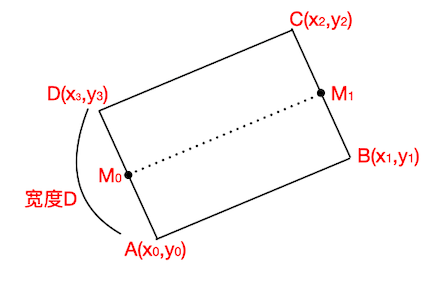
\includegraphics[width=12cm]{figures/obstacle_bottom.png}
    \caption{障碍物底面}
    \label{fig:obstacle_bottom}
\end{figure}
\par 特别注意特殊判断长宽平行与轴的情况,此时可以直接通过$M_0,M_1$的坐标计算四个顶点的坐标,即四个顶点的坐标分别为$(x_0,y_0-\dfrac{D}{2}),(x_0,y_0+\dfrac{D}{2}),(x_1,y_1-\dfrac{D}{2}),(x_1,y_1+\dfrac{D}{2})$。
具体的代码如图\ref{code:obstacle_vertice_process},通过if-else判断情况来具体计算,最后通过重载结构体的读入来实现使用c++的cin就可以读入障碍物数据时计算顶点并存储在结构体当中,方便后续使用。
其中结构体当中的conveyByPrec函数是将原始数据下的障碍物离散到指定precision精度下的处理后的障碍物。
\lstinputlisting[style=C++,caption={顶点处理},label=code:obstacle_vertice_process]{code/obstacle_vertice_process.cpp}
\par 通过处理数据,使得可以将最短路径算法应用在三维空间当中,通过控制离散化的精度来实现控制最短路径的精度,离散后格点的标记来实现不可访问情况的判断,达到将实际空间离散化到指定精度的理想空间,从而计算出格点组成的最短路径。

\subsection{相交判断}
\par 通过计算出格点组成的最短路径后,由于存在三角形定则,即三角形两边之和大于第三边,所以在计算的格点路径后,是可以通过运用三角形定则拟合计算出更短的路径,此时就需要判断所拟合的新路径是否经过了障碍物。此时问题可以抽象为线段与长方体是否相交的判定问题,根据线段的向量表示法,有线段$\vec{PQ}$:$P+k(Q-P),k\in [0,1]$,若存在与某个障碍物相交的情况,即存在k属于0~1之间,使得该点在障碍物之内。
考虑障碍物:底面$A(x_0,y_0),B(x_1,y_1),C(x_2,y_2),D(x_3,y_3)$,高的范围$[z_0,z_1]$。由于障碍物的高与z轴平行,故只需要考虑该障碍物由无数个矩形在z轴上堆叠而成。首先,我们讨论如何判断一个二维点坐标是否位于底面矩形当中,设该点坐标为$E(x,y)$,若该点在矩形内,则满足$\vec{AB}\times\vec{AE}*\vec{CD}\times\vec{CE}\ge 0$,若该式子成立则说明该点在边AB和边CD之间;同理,还需要成立$\vec{DA}\times\vec{DE}*\vec{BC}\times\vec{BE}\ge 0$,即该点在边DA和BC之间。两个条件需要同时满足,则说明该点在四条边之内,即在该矩形范围内。
\par 将问题放大到三维空间当中,该线段若与该障碍物有交点,则至少存在一个可行的k解满足E的坐标在障碍物内,则我们求出要与该障碍物相交时k值所取的范围,若存在有效范围,则表明该线段与该障碍物相交。
首先,对于z轴相交,设$\vec{R}=PQ=Q-P$为向量$PQ$的方向向量,则k的范围应在$k\in [0,1]$,对于障碍物的z轴所计算的k的取值为:$k_0=\dfrac{z_0-P.z}{R.z},k_1=\dfrac{z_1-P.z}{R.z}$,若$R.z<0$小于0时交换$k_0,k_1$的值。则$k_0\leq k_1$存在z轴可行解,否则无解。代码如下\ref{code:check_insect_zaxis},首先初始化k取值范围为[0,1],通过分别计算$z_0,z_1$对应的k取值来更新。
\lstinputlisting[style=C++,caption={计算z轴k取值},label=code:check_insect_zaxis]{code/check_insect_zaxis.cpp}
对于x、y所决定的k值的范围,需要计算的是该点在矩形内部的情况,则可以用到之前我们所讨论到的公式
\begin{equation}
    \vec{AB}\times\vec{AE}*\vec{CD}\times\vec{CE}\ge 0
\label{con:innerABandCD}
\end{equation}
和
\begin{equation}
    \vec{DA}\times\vec{DE}*\vec{BC}\times\vec{BE}\ge 0
\label{con:innerDAandBC}
\end{equation}
公式\ref{con:innerABandCD}和\ref{con:innerDAandBC}两者需要同时成立。针对可能出现该点在xy平面内是一个点的情况,即一条平行与z轴的线段,此时利用公式\ref{con:innerABandCD}和\ref{con:innerDAandBC}对该点做一个计算,若两公式都满足则说明该线段在xy平面的点在障碍物底面中之中,该部分代码如下\ref{code:check_insect_onepoint}。
\lstinputlisting[style=C++,caption={相交时单点的情况},label=code:check_insect_onepoint]{code/check_insect_onepoint.cpp}
对于线段$\vec{PQ}$能到达的点坐标E,有$E(P.x+k(Q.x-P.x),P.y+k(Q.y-P.y))$。将该点E坐标代入公式\ref{con:innerABandCD}中有
\begin{align*} 
    \vec{AB}\times\vec{AE} = {}& (x_1-x_0,y_1-y_0)\times(P.x+k(Q.x-P.x)-x_0,P.y+k(Q.y-P.y)-y_0) \\ 
    = {}& [(x_1-x_0)(Q.y-P.y)-(Q.x-P.x)(y_1-y_0)]k  \\ 
    &{} +(x_1-x_0)(P.y-y_0)-(P.x-x_0)(y_1-y_0) 
\end{align*}
我们设k的系数$a_1=(x_1-x_0)(Q.y-P.y)-(Q.x-P.x)(y_1-y_0)$,后的常数为$b_1=(x_1-x_0)(P.y-y_0)-(P.x-x_0)(y_1-y_0)$,则公式可化简为$\vec{AB}\times\vec{AE} = a_1k+b_1$。
\begin{align*} 
    \vec{CD}\times\vec{CE} = {}& (x_3-x_2,y_3-y_2)\times(P.x+k(Q.x-P.x)-x_2,P.y+k(Q.y-P.y)-y_2) \\ 
    = {}& [(x_3-x_2)(Q.y-P.y)-(Q.x-P.x)(y_3-y_2)]k  \\ 
    &{} +(x_3-x_2)(P.y-y_2)-(P.x-x_2)(y_3-y_2) 
\end{align*}
设k的系数为$a_2=(x_3-x_2)(Q.y-P.y)-(Q.x-P.x)(y_3-y_2)$,后的常数为$b_2=(x_3-x_2)(P.y-y_2)-(P.x-x_2)(y_3-y_2)$,则公式可化简为$\vec{CD}\times\vec{CE} = a_2k+b_2$。
则$\vec{AB}\times\vec{AE}*\vec{CD}\times\vec{CE}\ge 0$等价于方程$(a_1k+b_1)*(a_2k+b_2) \ge 0 = a_1a_2x^2+(a_1b_2+a_2b_1)x+b_1b_2 \ge 0$,即是二次函数求解的问题。
关于二次函数根求解的问题,我们需要讨论系数是否为0,以及特判二次函数出现非实数解的情况。若不存在这些情况,则对于二次函数$y=ax^2+bx+c$,二次函数根的计算公式:
\begin{equation}
    x=\dfrac{-b\pm\sqrt{b^2-4ac}}{2a}
\label{con:Quadratic_functions}
\end{equation}
故我们将公式\ref{con:Quadratic_functions}应用在方程$a_1a_2x^2+(a_1b_2+a_2b_1)x+b_1b_2 \ge 0$上,可以得到该方程的解为
\begin{equation}
    k=\dfrac{-(a_1b_2+a_2b_1)\pm\sqrt{(a_1b_2+a_2b_1)^2-4a_1a_2b_1b_2}}{2a_1a_2}
\label{con:kBaseOnQuadFun}
\end{equation}
我们将之前假设的$a_1,a_2,b_1,b_2$代入该公式既可以求出对于公式\ref{con:innerABandCD}限制下k的取值范围。使用该求解值更新基于z范围求出的k范围,若新的$k_0\leq k_1$则存在可行解,否则无解。代码如下\ref{code:check_insect_firstcross},代码首先判断了出现系数为0时二次函数退化为一次函数的情况,下文将进行分析,否则计算二次函数对应的k值用来更新并判断。
\lstinputlisting[style=C++,caption={公式\ref{con:innerABandCD}求解k值},label=code:check_insect_firstcross]{code/check_insect_firstcross.cpp}
\par 对于公式\ref{con:innerDAandBC},相似的有,我们将点E坐标代入有
\begin{align*} 
    \vec{DA}\times\vec{DE} = {}& (x_0-x_3,y_0-y_3)\times(P.x+k(Q.x-P.x)-x_3,P.y+k(Q.y-P.y)-y_3) \\ 
    = {}& [(x_0-x_3)(Q.y-P.y)-(Q.x-P.x)(y_0-y_3)]k  \\ 
    &{} +(x_0-x_3)(P.y-y_3)-(P.x-x_3)(y_0-y_3) 
\end{align*}
同样的,设k的系数$a_1=(x_0-x_3)(Q.y-P.y)-(Q.x-P.x)(y_0-y_3)$,后的常数为$b_1=(x_0-x_3)(P.y-y_3)-(P.x-x_3)(y_0-y_3)$,则公式可化简为$\vec{DA}\times\vec{DE} = a_1k+b_1$。
\begin{align*} 
    \vec{BC}\times\vec{BE} = {}& (x_2-x_1,y_2-y_1)\times(P.x+k(Q.x-P.x)-x_1,P.y+k(Q.y-P.y)-y_1) \\ 
    = {}& [(x_2-x_1)(Q.y-P.y)-(Q.x-P.x)(y_2-y_1)]k  \\ 
    &{} +(x_2-x_1)(P.y-y_1)-(P.x-x_1)(y_2-y_1) 
\end{align*}
设k的系数为$a_2=(x_2-x_1)(Q.y-P.y)-(Q.x-P.x)(y_2-y_1)$,后的常数为$b_2=(x_2-x_1)(P.y-y_1)-(P.x-x_1)(y_2-y_1)$,则公式可化简为$\vec{CD}\times\vec{CE} = a_2k+b_2$。
故我们将新的$a_1,a_2,b_1,b_2$的值代入公式\ref{con:kBaseOnQuadFun}中计算出对于公式\ref{con:innerDAandBC}限制下的k的取值范围。使用新求解的k值更新由公式\ref{con:innerABandCD}更新的k值,若最后求解的k值仍满足$k_0\leq k_1$,则说明线段$PQ$存在与该障碍物相交的情况。
具体代码如下\ref{code:check_insect_secondcross},代码同样先判断了退化的情况,再计算的二次函数对应k取值来更新并判断。若最后更新后的k取值仍满足$k_0\leq k_1$,则说明存在可行k解使得存在该线段$PQ$与障碍物相交,此时代码true表示产生碰撞。
\lstinputlisting[style=C++,caption={公式\ref{con:innerDAandBC}求解k值},label=code:check_insect_secondcross]{code/check_insect_secondcross.cpp}
\par 针对可能出现的二次函数系数为0的情况,即公式退化为一次函数的正负问题,如$b_1(a_2k+b_2)\ge 0$,此时特判系数为0的各种情况,计算一次函数下k的取值即可,代码如图\ref{code:check_insect_firstcross}的8行至20行。对于出现非实数解的情况,即$\Delta=b^2-4ac<0$时,此时表明不存在有效k的取值的点使之在障碍物内,故该线段与障碍物不相交。
\par 至此,已经完成了三维空间内线段与障碍物相交的讨论,利用通过离散化格点求解的格子点路径,不断检查格子点之间是否存在不与障碍物相交也能相连且距离更短的情况,来进一步优化路径。

\subsection{最短路径算法}
\par 三维空间最短路径算法的实现,在指定精度后,将实际空间离散到指定精度的空间,因此算法需要求解出离散空间中从起点到终点的格点最短路径,再利用上述讨论的相交算法来拟合路径,最后给出该精度下近似的最短路径和所通过的格点线段。
\subsubsection{基于BFS的三维最短路径算法}
\par 广度优先搜索(BFS)算法,又叫做宽度优先搜索,是一种在图上的搜索算法。算法将从根节点开始,沿着树的宽度遍历树的节点。在图上时,可以视为根节点为起点的一棵树。BFS是一种暴力算法,目的是系统的展开并检查图中的所有节点,以找寻结果。算法的实现一般采用open-closed表,所有因为展开节点而得到都会被加进一个先进先出的队列中,其邻居节点尚未检验的节点会被存放在一个称为open的容器,而被检验过的节点则被存放在被称为closed的容器中。其实现方法为:
\begin{enumerate}
    \item 首先将根节点放在队列中。
    \item 从队列中取出现在的第一个节点,并检查。
    \begin{itemize}
        \item 如果找到目标,则结束搜索并返回结果。
        \item 否则将它所有还没有检查过的相邻子节点加入队列中。
    \end{itemize}
    \item 若队列为空,表示检查了所有点都没有找到目标。结束搜索并返回未找到目标。
    \item 重复步骤2.
\end{enumerate}
\par 在离散后的三维空间中,将把每一个整数格点视为顶点,即$V=\{v_i(x,y,z)|x\in N,y\in N,z\in N\}$,则对于顶点$v_1=(x,y,z)$相邻的顶点有分别在x轴、y轴、z轴相邻的6个顶点:$(x-1,y,z),(x+1,y,z),(x,y-1,z),(x,y+1,z),(x,y,z-1),(x,y,z+1)$。
则基于BFS的三维空间最短路径算法实现,是基于从起点格点逐渐向外发散并记录所经过的路径,直到找到终点。算法需要遍历大量的点,若起点$st(x_0,y_0,z_0)$与终点$ed(x_1,y_1,z_1)$之间三维坐标差的最大值为$n=max\{x_1-x_0,y_1-y_0,z_1-z_0\}$,则算法至少需要遍历$n^3$个点,则算法的时间复杂度为$O(n^3)$,空间复杂度为$O(n^3)$。
搜索算法初始化部分如代码\ref{code:bfs_init}所示,首先定义了距离向量dist,用来存储起点距离该格点的最短路径的长度;方向向量dir,用来找到现在顶点相邻的顶点;以及使用数组q和指针front和rear实现队列的功能,并能将顶点保存起来用来回溯路径;pre数组存储该顶点nowNode的前驱顶点preNode,即是BFS时nowNode是通过preNode搜索到的且经过格子点数量最少的情况时的前驱顶点。
\lstinputlisting[style=C++,caption={BFS搜索算法初始化代码},label=code:bfs_init]{code/bfs_alorithm_init.cpp}
\par 初始化完成后,算法使用数组实现的队列q,front指针表示当前节点在队列中的位置,rear指针表示队列的最后一个节点的位置,当$front\leq rear$时表示队列不为空。则算法通过不断取出队列的当前节点,并检查是否为终点,或者跳过路径长度以及大于了已经找到的最短路径长度的节点,对搜索做剪枝。随后遍历该节点的相邻节点,若相邻节点没有超出边界且可以访问,则更新其距离向量,并将其加入到队列中。
\lstinputlisting[style=C++,caption={BFS搜索算法主要代码},label=code:bfs_main]{code/bfs_alorithm.cpp}
\par 若算法返回true则代表至少存在一条从起点格点到终点格点的格点最短路径,此时需要我们对路径做一个拟合,进一步优化路径长度。根据上述障碍物相交判断中所实现的函数check_insect做该条路径上顶点到顶点的拟合操作,即若直接在这两个顶点之间连成线段不经过障碍物且距离更短。此时拟合算法所需要的时间与所找到的最短路径长度有关,对于BFS搜索算法,平均最短路径上的格子节点在$$
\subsubsection{基于A*的三维最短路径算法}

\section{本章总结}
